\section{Introduction}

%% Background
In this paper, we study streaming analytics in the wide area, where the data
generating sites are different from data processing sites. Such data is most
valuable if we can transport, distill and analyze in real time. For example, a
content distribution network (CDN) analyzes the logs from geo-distributed
infrastructure to optimize content placement. Recently, the emerging class of
Internet of Things (IoT) applications makes the wide-area streaming analytical
workload even more important. Large cities such as New York, Beijing and Seattle
have deployed millions of cameras for traffic
control~\cite{london.surveillance,skynet}. Our buildings are increasingly
equipped with a wide variety of sensors to improve building energy use, occupant
comfort, reliability and maintenance~\cite{krioukov2012building}.

While existing stream processing systems, such as Spark
Streaming~\cite{zaharia2013discretized}, and specialized analytical engines,
such as VideoStorm~\cite{zhang2017live}, are capable of handling large streams
of data, they are designed to work within a single cluster. Within a single
cluster, there is sufficient bandwidth between worker nodes; in contrast the
wide area has scarce and variable bandwidth~\cite{hsieh17gaia,
  vulimiri2015global}. Back-hauling all the data across the wide-area is neither
viable nor efficient. The growth of the wide-area bandwidth has been
decelerating for many years~\cite{global2016telegeography} while the traffic
grows at a staggering rate~\cite{index2013zettabyte}. On the efficiency side,
raw data often contains large and less relevant details that can be aggregated,
pruned or compressed~\cite{rabkin2014aggregation}.

Pushing computations towards the edge is a key techinque to reduce bandwidth
requirement in recent WAN-aware systems~\cite{satyanarayanan2009case,
  rabkin2014aggregation, pu2015low}. However, communications are not entirely
avoidable for the following reasons: (i) the analytics require joining or
aggregating data from multiple geo-distributed
sites~\cite{viswanathan2016clarinet}; (ii) the edge can benefit significantly
from central computing resources such as GPU or TPU~\cite{norm2016google} in the
cloud; (iii) end-devices, such as cameras or mobile devices, also suffer from
the bandwidth in the last-hop wireless link~\cite{zhang2015design,
  abari2017enabling}.

% could improve efficiency (such as GDA pushes queries out; cloudlet
% etc). However, we still need data transmission for cloud off-loading or
% aggregation purpose.

When facing insufficient bandwidth, application developers need to make a
decision within the design space of data freshness and data fidelity
(\autoref{fig:intro}):

\begin{figure}
  \centering
  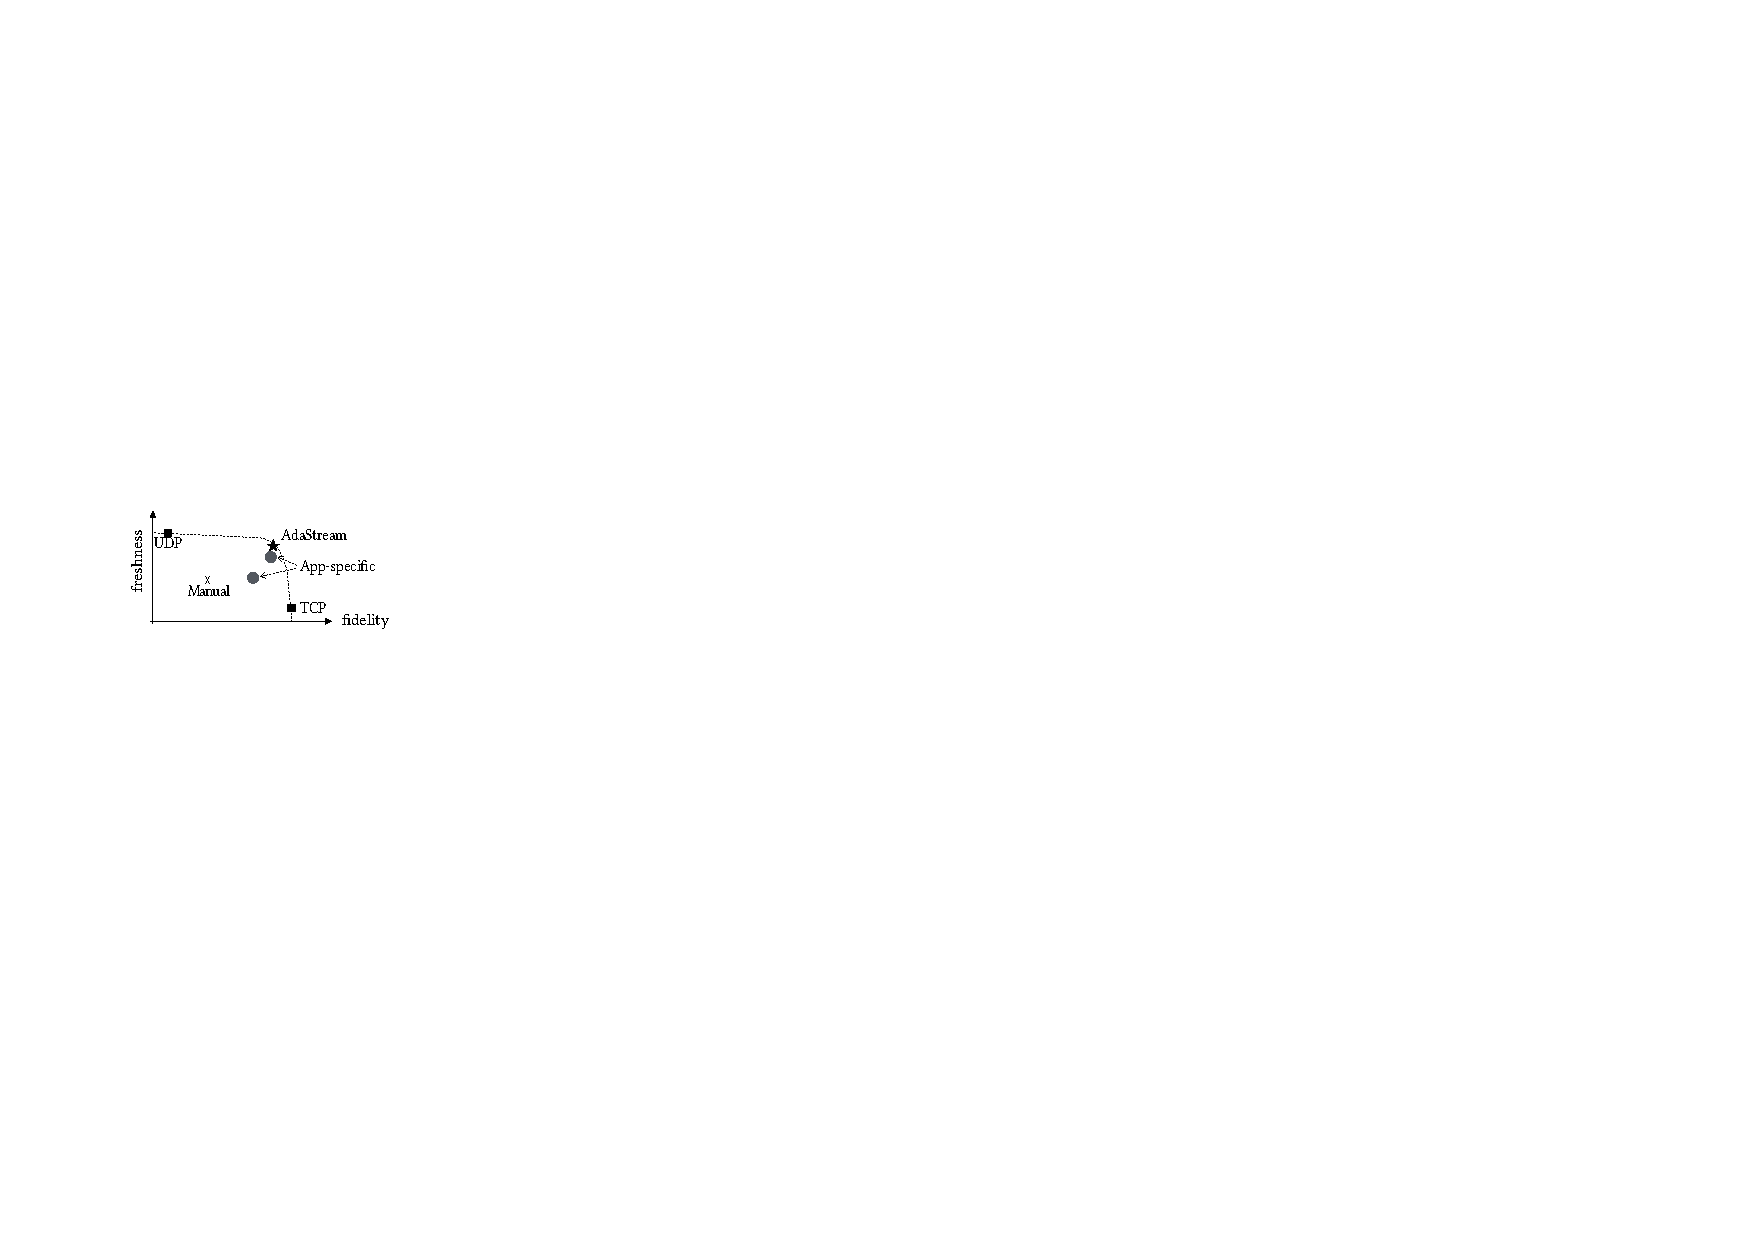
\includegraphics[width=0.9\linewidth]{figures/intro.pdf}
  \caption{The trade-off space between data freshness and data fidelity when
    facing insufficient bandwidth.}
  \label{fig:intro}
  \vspace{-1em}
\end{figure}

(i) Existing transport protocols often choose one extreme point in the design
space. Building applications with TCP ensures a reliable delivery of the data
but the backlogged data will increase application latency. Building applications
with UDP minimizes latency by sending packets as fast as possible, but the
uncontrolled packet loss along the network may devastate the application.

(ii) Manual policies, such as sampling, can trade data fidelity for
freshness~\cite{rabkin2014aggregation}. However, these policies are often
developer heuristics without measurements backing up. An accurate policy often
requires extensive developer efforts or domain expertise. Inaccurate policies,
in practice, provide sub-optimal performance in both freshness and fidelity.

(iii) Application-specific optimizations do not generalize. One trade-off
strategy designed to work well for one application under one condition renders
sub-optimal performances when the scenario changes. For example, video streaming
delivers videos for human consumption and focuses on Quality of Experience
(QoE)~\cite{yin2015control}. As a consequence, optimal adaptations favor
smoothness over image quality, i.e., 25 frames per second (FPS) or higher. Such
strategies fail to explore adaptations with a smaller FPS for machine-based
video analytics.

In this paper, we present \sysname{}, the first stream processing system for the
wide area that addresses the bandwidth limitations with a system-level
solution. At the core, \sysname{} integrates application adaptation as a
first-class abstraction within the stream processing model and allows an
accurate trade-off exploration between data fidelity and freshness.

We propose an \maybe{} operator as part of the stream processing
application. \maybe{} takes a list of values as a knob and a function that
transforms an input stream into a degraded stream. Our APIs offer a number of
advantages over existing approaches. (i) Developers are not assume to be experts
in the application domain. Instead of writing exact policies, developers only
need to hint at potential operations. For example, while a developer may not
understand how downsampling the video affects either data rate or object
detection accuracy, she can express the downsample operation with a few
resolution options using \maybe APIs. (ii) \sysname{}'s APIs are modular and
extensible. Custom functions from external libraries be embedded inside the
operator. We can also specialize the basic operator by providing degradation
functions for common data types, such as \texttt{maybe\_head} for a list or
\texttt{maybe\_downsample} for images.  (iii) The similarity with other
operators makes it easy to integrate with existing stream processing systems.
We name our approach \textit{structured adaptation} to contrast from existing
adaptations with ad-hoc policies.

\sysname{} then uses a data-driven approach to learn the application performance
for different levels of degradation. The combination of all \maybe{} operators
form a \textit{configuration} that affects bandwidth demand and application
accuracy. By profiling with representative training data and an
application-specific accuracy function, \sysname{} explores the configuration
space automatically to learn a Pareto-optimal adaptation strategy. The strategy,
or \textit{profile}, contains configurations that can achieve the highest
accuracy for a given bandwidth constrain. We support both offline and online
profiling; and speed up using a number of techniques, such as parallelism and
reduce the profiling workload with partial profiling.

At runtime, \sysname{} monitors the application execution and adapt the
application execution such that the application's data rate matches the
available bandwidth. Because the learned profile consists of discrete
configurations, the level of data rate changes may be coarse. We propose a novel
probe-based control for fine-grain bandwidth estimation. When multiple streams
share the same bottle-neck link, the learned profiles can be used for allocating
bandwidth resources. While existing systems can only achieve bandwidth-fairness,
\sysname{} supports utility-fairness that maximizes the minimal accuracy.

To evaluate \sysname{}, we've built three streaming applications: pedestrian
detection (PD), augmented reality (AR) and a distributed Top-K (TK) analysis. We
use real-world data (existing or collected) to evaluate these applications for
the profiling and runtime systems. The evaluation results and our contributions
are summarized as follows:

\begin{itemize}[leftmargin=16pt]
\item We design and implement \sysname{}, the first stream processing system
  that simultaneously achieves low latency and high accuracy. We build three
  real-world applications and evaluate the performance extensively.
\item We propose to integrate adaptation as a first-class abstraction in stream
  processing. Such a programming abstraction requires minimal developer efforts,
  is extensible and allows easy integration with existing frameworks.
\item We employ a data-driven approach to learn an accurate and precise profile
  both at offline and online. To allow an efficient profiling without losing
  generality, we evaluate the potential speed ups with parallelism and partial
  profiling.
\item We demonstrate the profile allows the runtime to adapt application
  execution to match available bandwidth, achieving low latency while
  maintaining high accuracy. In our experiments, \sysname{} applications achieve
  sub-second latency with nominal accuracy drop.
\end{itemize}

%%% Local Variables:
%%% mode: latex
%%% TeX-master: "sosp17"
%%% End:

%% LocalWords: VideoStorm, analytics, CDN, IoT
